\documentclass{article}


% if you need to pass options to natbib, use, e.g.:
%     \PassOptionsToPackage{numbers, compress}{natbib}
% before loading neurips_2023


% ready for submission
%\usepackage{neurips_2023}
\usepackage[final]{neurips_2023}

% to compile a preprint version, e.g., for submission to arXiv, add add the
% [preprint] option:
%     \usepackage[preprint]{neurips_2023}


% to compile a camera-ready version, add the [final] option, e.g.:
%     \usepackage[final]{neurips_2023}


% to avoid loading the natbib package, add option nonatbib:
%    \usepackage[nonatbib]{neurips_2023}


\usepackage[utf8]{inputenc} % allow utf-8 input
\usepackage[T1]{fontenc}    % use 8-bit T1 fonts
\usepackage{hyperref}       % hyperlinks
\usepackage{url}            % simple URL typesetting
\usepackage{booktabs}       % professional-quality tables
\usepackage{amsfonts}       % blackboard math symbols
\usepackage{nicefrac}       % compact symbols for 1/2, etc.
\usepackage{microtype}      % microtypography
\usepackage{xcolor}         % colors
\usepackage{graphicx}

\title{Improving PPI Prediction with ESMC-derived Features}


% The \author macro works with any number of authors. There are two commands
% used to separate the names and addresses of multiple authors: \And and \AND.
%
% Using \And between authors leaves it to LaTeX to determine where to break the
% lines. Using \AND forces a line break at that point. So, if LaTeX puts 3 of 4
% authors names on the first line, and the last on the second line, try using
% \AND instead of \And before the third author name.



\author{
	Anrui Wang \\
	2023000000 \\
	\texttt{wangar2023@shanghaitech.edu.cn}\\
	\AND
	Jiawen Dai \\
	2023533132 \\
	\texttt{daijw2023@shanghaitech.edu.cn}\\
	 \AND
	 Yiting Qi \\
	 2023000000 \\
	 \texttt{qiyt2023@shanghaitech.edu.cn}\\
}


\begin{document}
	
	
	\maketitle
	
	
	\begin{abstract}
		The abstract paragraph should be indented \nicefrac{1}{2}~inch (3~picas) on
		both the left- and right-hand margins. Use 10~point type, with a vertical
		spacing (leading) of 11~points.  The word \textbf{Abstract} must be centered,
		bold, and in point size 12. Two line spaces precede the abstract. The abstract
		must be limited to one paragraph.
	\end{abstract}
	
	
	\section{Introduction}

	
	111
	
	
	\subsection{Research background}
	
	
	the method b4ppi use
	
	
	\subsection{Motivation}
	
	
	we want to use embeddings from esmC
	
	
	\paragraph{Preprint option}
	111
	
	
	\section{Methods}

	\subsection{Embedding extraction}
	\subsection{Data Processing}

	Prior to feeding the protein embeddings into the supervised learning network, we first standardized the dimensionality by processing the original $(L+2) \times 960$ matrices into uniform representations.
	
	\paragraph{Average pooling} We first implemented {average pooling} and {max pooling} along the sequence dimension ($L+2$), compressing each sequence into a fixed-size embedding of $[1, 960]$. While these two approaches successfully standardize input dimensions and reduce computational overhead by handling large embedding matrices, they inherently discards critical positional and structural information.
	
	\paragraph{Masked Autoencoder (MAE)} To overcome the limitation above, we subsequently developed a {Masked Autoencoder} framework with standardized sequence lengths ($L = 1502$), employing zero-padding for shorter sequences and truncation for longer ones. 
	This method incorporates a 75\% masking rate during training, though initial experiments revealed issues with low data variance and interference from padded positions. The model suffers from small loss and learning wrong pattern from the padding position.
	
	 These challenges were mitigated through feature normalization and by restricting loss computation to non-padding regions. We normalize every protein embedding matrix to have a variance equal to 1, as well as replace L2 loss with L1 loss. A key refinement involved explicitly marking padding boundaries (adding a variable \texttt{padding\_start}) and implementing a 50\% masking strategy exclusively on non-padded segments, ensuring more focused learning. The model's architecture, which now processes structured inputs containing both sequence data and padding metadata, demonstrates improved convergence. This combined approach effectively balances dimensionality reduction with information preservation, whose result is better than average pooling and max pooling as expected.
	
The provided figure illustrates the reconstruction performance of our Masked Autoencoder (MAE) framework on protein sequence embeddings at training epoch 60. The visualization compares the original feature values (blue line), reconstructed values (orange line), and masked positions (red crosses) across the standardized sequence length of 1502.

% Three key observations emerge from this analysis:
%		
%		First, the reconstruction fidelity demonstrates the model's ability to recover meaningful patterns from heavily masked inputs (75\% masking rate during training). The close alignment between original and reconstructed values in unmasked regions (e.g., positions 400-600) indicates successful learning of sequence features, while deviations at masked positions (red crosses) reflect the model's probabilistic reconstruction behavior.
%		
%		Second, the implementation details shown in the code snippet - particularly the handling of sequence lengths through \texttt{sample\_len} and \texttt{mask\_bool\_vis} - enable precise masking application only to non-padding regions. This explains the consistent reconstruction quality throughout the active sequence portion (approximately first 1000 positions), with potential degradation near the padding boundary (position 1502 not shown).
%		
%		Third, the standardized length treatment (zero-padding and truncation to $L=1502$) combined with our 50\% non-padding masking strategy produces stable gradients, as evidenced by the smooth reconstructed curve. The \texttt{padding\_start} metadata prevents the model from learning artificial padding patterns, while the selective masking concentrates learning on biologically relevant sequence segments.
%		
%		This visualization confirms our methodological improvements over pooling approaches, showing both global pattern retention (through the overall curve similarity) and local detail recovery (visible in high-frequency feature variations). The remaining reconstruction errors primarily occur at masked positions, suggesting appropriate model uncertainty rather than systematic failure.

	\paragraph{Compress first and then splice} 
	
	\begin{figure}[h]
		\centering
		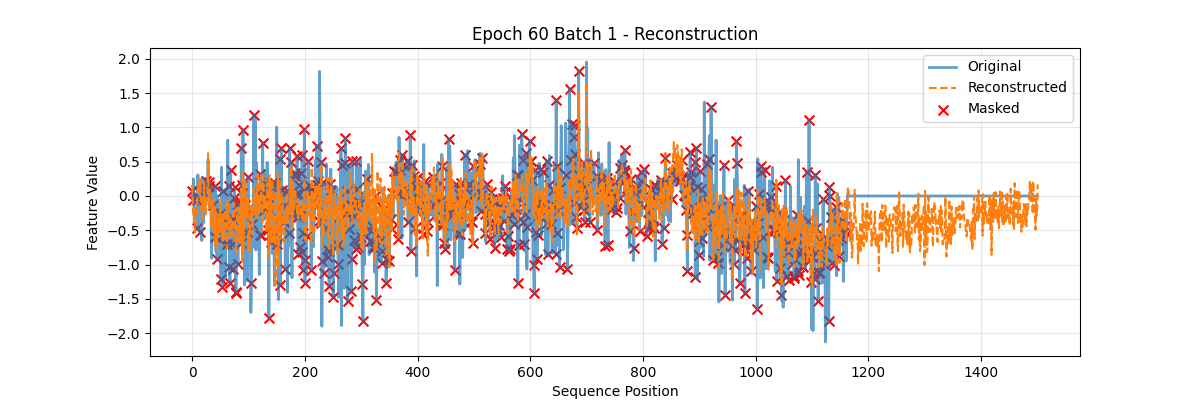
\includegraphics[width=0.7\textwidth]{imgs/epoch60_batch1.png}
		\caption{A recon of protein embedding from MAE}
		% \label{fig:datasheet_page3}
	\end{figure}
	
 Our experiments demonstrate that {feature compression prior to concatenation yields superior efficacy} compared to post-concatenation compression. The latter approach — initially concatenating protein features followed by compression — was motivated by the hypothesis that Masked Autoencoders (MAE) might capture inter-protein dependencies during compression. However, due to computational constraints, we truncated concatenated protein embeddings to a maximum length of 2000. Preliminary attempts employing this methodology resulted in performance degradation, potentially attributable to extreme sequence length disparities: when merging proteins with widely varying lengths (e.g., 1000 vs. 40 amino acids). Length heterogeneity may force suboptimal compromises in the attention distribution during compression.  
	
	
	\subsection{Supervised learning}

 We formulate protein-protein interaction prediction as a binary classification task by first compressing individual protein sequences into fixed-length embeddings using our MAE framework, then constructing paired samples through vector concatenation ($\mathbf{x} = [\mathbf{e}_i \|\mathbf{e}_j] \in \mathbb{R}^{1920}$). These embedding pairs, labeled with interaction status (1/0), train a supervised classifier to predict novel interactions. This approach maintains structural information while enabling efficient pairwise analysis.
	
	\section{Experiments}
	
	\subsection{L2-cos Method}
	High similarity between proteins does not necessarily imply that they have a PPI.
	
	\subsection{Logistic Regression}
	\subsection{XGBoost}
	\subsection{Multi-Layer Perceptron (MLP)}
	
	
	\section{Conclusion}
	\subsection{Future work}
111
	
\section{example}
	\begin{center}
		\url{http://mirrors.ctan.org/macros/latex/contrib/natbib/natnotes.pdf}
	\end{center}
	Of note is the command \verb+\citet+, which produces citations appropriate for
	use in inline text.  For example,
	\begin{verbatim}
		\citet{hasselmo} investigated\dots
	\end{verbatim}
	produces
	\begin{quote}
		Hasselmo, et al.\ (1995) investigated\dots
	\end{quote}
	
	
	If you wish to load the \verb+natbib+ package with options, you may add the
	following before loading the \verb+neurips_2023+ package:
	\begin{verbatim}
		\PassOptionsToPackage{options}{natbib}
	\end{verbatim}
	
	
	If \verb+natbib+ clashes with another package you load, you can add the optional
	argument \verb+nonatbib+ when loading the style file:
	\begin{verbatim}
		\usepackage[nonatbib]{neurips_2023}
	\end{verbatim}
	
	
	As submission is double blind, refer to your own published work in the third
	person. That is, use ``In the previous work of Jones et al.\ [4],'' not ``In our
	previous work [4].'' If you cite your other papers that are not widely available
	(e.g., a journal paper under review), use anonymous author names in the
	citation, e.g., an author of the form ``A.\ Anonymous'' and include a copy of the anonymized paper in the supplementary material.
	
	
	\subsection{Footnotes}
	
	
	Footnotes should be used sparingly.  If you do require a footnote, indicate
	footnotes with a number\footnote{Sample of the first footnote.} in the
	text. Place the footnotes at the bottom of the page on which they appear.
	Precede the footnote with a horizontal rule of 2~inches (12~picas).
	
	
	Note that footnotes are properly typeset \emph{after} punctuation
	marks.\footnote{As in this example.}
	
	
	\subsection{Figures}
	
	
	\begin{figure}
		\centering
		\fbox{\rule[-.5cm]{0cm}{4cm} \rule[-.5cm]{4cm}{0cm}}
		\caption{Sample figure caption.}
	\end{figure}
	
	
	All artwork must be neat, clean, and legible. Lines should be dark enough for
	purposes of reproduction. The figure number and caption always appear after the
	figure. Place one line space before the figure caption and one line space after
	the figure. The figure caption should be lower case (except for first word and
	proper nouns); figures are numbered consecutively.
	
	
	You may use color figures.  However, it is best for the figure captions and the
	paper body to be legible if the paper is printed in either black/white or in
	color.
	
	
	\subsection{Tables}
	
	
	All tables must be centered, neat, clean and legible.  The table number and
	title always appear before the table.  See Table~\ref{sample-table}.
	
	
	Place one line space before the table title, one line space after the
	table title, and one line space after the table. The table title must
	be lower case (except for first word and proper nouns); tables are
	numbered consecutively.
	
	
	Note that publication-quality tables \emph{do not contain vertical rules.} We
	strongly suggest the use of the \verb+booktabs+ package, which allows for
	typesetting high-quality, professional tables:
	\begin{center}
		\url{https://www.ctan.org/pkg/booktabs}
	\end{center}
	This package was used to typeset Table~\ref{sample-table}.
	
	
	\begin{table}
		\caption{Sample table title}
		\label{sample-table}
		\centering
		\begin{tabular}{lll}
			\toprule
			\multicolumn{2}{c}{Part}                   \\
			\cmidrule(r){1-2}
			Name     & Description     & Size ($\mu$m) \\
			\midrule
			Dendrite & Input terminal  & $\sim$100     \\
			Axon     & Output terminal & $\sim$10      \\
			Soma     & Cell body       & up to $10^6$  \\
			\bottomrule
		\end{tabular}
	\end{table}
	
	\subsection{Math}
	Note that display math in bare TeX commands will not create correct line numbers for submission. Please use LaTeX (or AMSTeX) commands for unnumbered display math. (You really shouldn't be using \$\$ anyway; see \url{https://tex.stackexchange.com/questions/503/why-is-preferable-to} and \url{https://tex.stackexchange.com/questions/40492/what-are-the-differences-between-align-equation-and-displaymath} for more information.)
	
	\subsection{Final instructions}
	
	Do not change any aspects of the formatting parameters in the style files.  In
	particular, do not modify the width or length of the rectangle the text should
	fit into, and do not change font sizes (except perhaps in the
	\textbf{References} section; see below). Please note that pages should be
	numbered.
	
	
	\section{Preparing PDF files}
	
	
	Please prepare submission files with paper size ``US Letter,'' and not, for
	example, ``A4.''
	
	
	Fonts were the main cause of problems in the past years. Your PDF file must only
	contain Type 1 or Embedded TrueType fonts. Here are a few instructions to
	achieve this.
	
	
	\begin{itemize}
		
		
		\item You should directly generate PDF files using \verb+pdflatex+.
		
		
		\item You can check which fonts a PDF files uses.  In Acrobat Reader, select the
		menu Files$>$Document Properties$>$Fonts and select Show All Fonts. You can
		also use the program \verb+pdffonts+ which comes with \verb+xpdf+ and is
		available out-of-the-box on most Linux machines.
		
		
		\item \verb+xfig+ "patterned" shapes are implemented with bitmap fonts.  Use
		"solid" shapes instead.
		
		
		\item The \verb+\bbold+ package almost always uses bitmap fonts.  You should use
		the equivalent AMS Fonts:
		\begin{verbatim}
			\usepackage{amsfonts}
		\end{verbatim}
		followed by, e.g., \verb+\mathbb{R}+, \verb+\mathbb{N}+, or \verb+\mathbb{C}+
		for $\mathbb{R}$, $\mathbb{N}$ or $\mathbb{C}$.  You can also use the following
		workaround for reals, natural and complex:
		\begin{verbatim}
			\newcommand{\RR}{I\!\!R} %real numbers
			\newcommand{\Nat}{I\!\!N} %natural numbers
			\newcommand{\CC}{I\!\!\!\!C} %complex numbers
		\end{verbatim}
		Note that \verb+amsfonts+ is automatically loaded by the \verb+amssymb+ package.
		
		
	\end{itemize}
	
	
	If your file contains type 3 fonts or non embedded TrueType fonts, we will ask
	you to fix it.
	
	
	\subsection{Margins in \LaTeX{}}
	
	
	Most of the margin problems come from figures positioned by hand using
	\verb+\special+ or other commands. We suggest using the command
	\verb+\includegraphics+ from the \verb+graphicx+ package. Always specify the
	figure width as a multiple of the line width as in the example below:
	\begin{verbatim}
		\usepackage[pdftex]{graphicx} ...
		\includegraphics[width=0.8\linewidth]{myfile.pdf}
	\end{verbatim}
	See Section 4.4 in the graphics bundle documentation
	(\url{http://mirrors.ctan.org/macros/latex/required/graphics/grfguide.pdf})
	
	
	A number of width problems arise when \LaTeX{} cannot properly hyphenate a
	line. Please give LaTeX hyphenation hints using the \verb+\-+ command when
	necessary.
	
	
	\begin{ack}
		Use unnumbered first level headings for the acknowledgments. All acknowledgments
		go at the end of the paper before the list of references. Moreover, you are required to declare
		funding (financial activities supporting the submitted work) and competing interests (related financial activities outside the submitted work).
		More information about this disclosure can be found at: \url{https://neurips.cc/Conferences/2023/PaperInformation/FundingDisclosure}.
		
		
		Do {\bf not} include this section in the anonymized submission, only in the final paper. You can use the \texttt{ack} environment provided in the style file to autmoatically hide this section in the anonymized submission.
	\end{ack}
	
	
	
	\section{Supplementary Material}
	
	Authors may wish to optionally include extra information (complete proofs, additional experiments and plots) in the appendix. All such materials should be part of the supplemental material (submitted separately) and should NOT be included in the main submission.
	
	
	\section*{References}
	
	
	References follow the acknowledgments in the camera-ready paper. Use unnumbered first-level heading for
	the references. Any choice of citation style is acceptable as long as you are
	consistent. It is permissible to reduce the font size to \verb+small+ (9 point)
	when listing the references.
	Note that the Reference section does not count towards the page limit.
	\medskip
	
	
	{
		\small
		
		
		[1] Alexander, J.A.\ \& Mozer, M.C.\ (1995) Template-based algorithms for
		connectionist rule extraction. In G.\ Tesauro, D.S.\ Touretzky and T.K.\ Leen
		(eds.), {\it Advances in Neural Information Processing Systems 7},
		pp.\ 609--616. Cambridge, MA: MIT Press.
		
		
		[2] Bower, J.M.\ \& Beeman, D.\ (1995) {\it The Book of GENESIS: Exploring
			Realistic Neural Models with the GEneral NEural SImulation System.}  New York:
		TELOS/Springer--Verlag.
		
		
		[3] Hasselmo, M.E., Schnell, E.\ \& Barkai, E.\ (1995) Dynamics of learning and
		recall at excitatory recurrent synapses and cholinergic modulation in rat
		hippocampal region CA3. {\it Journal of Neuroscience} {\bf 15}(7):5249-5262.
	}
	
	%%%%%%%%%%%%%%%%%%%%%%%%%%%%%%%%%%%%%%%%%%%%%%%%%%%%%%%%%%%%
	
	
\end{document}